\documentclass[10pt, a4paper]{article}
\usepackage[top=0.6in,bottom=1.0in,left=1.0in,right=1.0in]{geometry}
\usepackage{amsmath,amssymb}
\usepackage{hyperref}
\usepackage{graphicx,float,tikz}
\usepackage{listings}
\fontfamily{times}

\title{\large CS 4366: Senior Capstone Project \\ Dr. Sunho Lim \\ Project \#4 - Implementation and Partial Demo - Project Report \\ EmergenSeek}
\author{Suhas Bacchu \ Derek Fritz \ Kevon Manahan \ Annie Vo \ Simon Woldemichael}
\date{April 1, 2019}

\begin{document}

\maketitle
\vspace{-1cm}
\begin{abstract}
In this report, we describe and detail the progress that we have made so far in developing the backend and mobile client for the EmergenSeek application. The report will be broken up into sections such that, each section will answer the questions posed in the \textbf{``Deliverables''} section of the Project 4 statement file.
\end{abstract}

\section{Project Restatement} 
\label{sec:pr}
As a reminder, EmergenSeek is a mobile application which will provide users with multiuse, centralized emergency information and notification services. This application will provide friends and family members with priority connections in times of emergency or crisis. For the scope of the following two months, within this class, our main function requirements are as follows.
\begin{enumerate}
	\item[1.] S.O.S. button emergency broadcast --- The user shall be able to utilize the mobile client to press and hold an S.O.S. button for automated notification of contacts and emergency services.
	\item[2.] Emergency service locator --- The user shall be able to utilize the mobile client to search for emergency service (i.e. hospitals, pharmacies, police boxes)
	\item[3.] Periodic notifications to contacts (location-based polling) --- The user shall be able to utilize the mobile client to periodically send their location information to contacts.
	\item[4.] Granular permission definitions for contacts --- The user shall be given full control over what contacts receive what level of information.
	\item[5.] Lock screen display of health information for emergency services --- In the case of an S.O.S. situation, the user shall have their health information displayed for the convince of first responders.
\end{enumerate}

\section{Lambda Functions}
\label{sec:lf}
\par ~ This section should be used as a reference when there is any mention of an implemented Lambda function. The functions are prefixed with \texttt{ES} (short for EmergenSeek). Please note that every instance of \texttt{user\_id} is a Universally unique identifier (UUID) generated by Firebase Auth (managed by the Flutter client). This section will detail 6 things for each Lambda function:
	\begin{enumerate}
		\item[1.] The HTTP method necessary for interacting with the Lambda function.
		\item[2.] The API Gateway route associated with the function.
		\item[3.] The JavaScript Object Notation (JSON) \underline{request} body required by the function to produce desired output.
		\item[4.] The JSON \underline{response} returned by the API for a request.
		\item[5.] A simple-to-understand description of what the function performs as a result of the request.
		\item[6.] Services and API's that this function is dependent upon.
	\end{enumerate}
	
	\pagebreak
	\begin{enumerate}
	%% ESSendSMSNotification
	\item[a.] \textbf{ESSendSMSNotification}
		\begin{itemize}		
		\item[(i)] HTTP Method: POST
		\item[(ii)] API Gateway Route: /sms
		\item[(iii)] JSON Request Body:
			\begin{lstlisting}
{
	"user_id": String
	"type": int,
	"message": String
	"last_known_location": double[2]
}
			\end{lstlisting}
		\item[(iv)] JSON Response Body (Success):
			\begin{lstlisting}
{
	"body": String
}
			\end{lstlisting}
		\item[(v)] Description: First, this function will update the user's location in the database. Second, If the user provides 1 as an emergency type (SEVERE) this function will send an SMS message to the user's primary and secondary contacts and send a voice call to emergency services. If the user provides 2 as an emergency type (MILD) this function will only send an SMS message to the user's primary contacts. If the user provides 3 as an emergency type (CHECKIN) this function will only send an SMS message to the user's primary contacts with the contents of the "message" field. The "message" field is only required if "type" is 3. The response body of this function, on success, is simply a string stating that all operations completed successfully.
		\item[(vi)] Dependencies: DynamoDB, Twilio
		\end{itemize}
		
	%% ESSendEmergencyVoiceCall
	\item[b.] \textbf{ESSendEmergencyVoiceCall}
		\begin{itemize}		
		\item[(i)] HTTP Method: POST
		\item[(ii)] API Gateway Route: /voice
		\item[(iii)] JSON Request Body:
			\begin{lstlisting}
{
    "user_id": String,
    "last_known_location": double[2]
}
			\end{lstlisting}
		\item[(iv)] JSON Response Body (Success):
			\begin{lstlisting}
{
	"body": String
}
			\end{lstlisting}
		\item[(v)] Description: First, this function will update the user's location in the database. Second, the application will generate an XML document which conforms to Twilio's TwilML (Twilio Markup Language) specification \cite{two}. This document specifies how the programmable voice call is programmed. Third, this application will uplaod the XML document to Amazon's Simple Storage Service so that Twilio may access it for every phonecall that is dispatched as a result of a single request to this Lambda function. Lastly, this function will call the user's primary contacts. Currently, we have not integrated anything which will determine the correct 911 phone number depending on the user's location. The response body of this function, on success, is simply a string stating that all operations completed successfully.
		\item[(vi)] Dependencies: DynamoDB, Twilio, Simple Storage Service
		\end{itemize}
		
	%% ESPollLocation
	\item[c.] \textbf{ESPollLocation}
		\begin{itemize}		
		\item[(i)] HTTP Method: POST
		\item[(ii)] API Gateway Route: /poll
		\item[(iii)] JSON Request Body:
			\begin{lstlisting}
{
    "user_id": String,
    "last_known_location": double[2]
}
			\end{lstlisting}
		\item[(iv)] JSON Response Body (Success):
			\begin{lstlisting}
{
	"body": String
}
			\end{lstlisting}
		\item[(v)] Description: First, this function will update the user's location in the database. Next, this function will utilize MapQuest's Geocoding API to translate the provided latitude and longitude into a readable address. Lastly, this function will send this updated location, in readable address format, to the user's primary and secondary contacts. The decision to use MapQuest instead of Google's Geocoding API was made as a result of there being a very friendly Golang library to take care of the all of the client code (\url{https://github.com/jasonwinn/geocoder}). The response body of this function, on success, is simply a string stating that all operations completed successfully.
		\item[(vi)] Dependencies: DynamoDB, Twilio, MapQuest
		\end{itemize}
	
	%% ESGetLockScreenInfo
	\item[d.] \textbf{ESGetLockScreenInfo}
		\begin{itemize}		
		\item[(i)] HTTP Method: POST
		\item[(ii)] API Gateway Route: /lock
		\item[(iii)] JSON Request Body:
			\begin{lstlisting}
{
    "user_id": String,
}
			\end{lstlisting}
		\item[(iv)] JSON Response Body (Success):
			\begin{lstlisting}
{
    "first_name": String,
    "last_name":  String,
    "blood_type": String,
    "age": int,
    "primary_residence": {
      "line1": String,
      "line2": String,
      "city": String,
      "state": String,
      "country": String,
      "zip_code": String
    },
    "phone_pin": int,
    "email_address": String,
    "phone_number": String
}
			\end{lstlisting}
		\item[(v)] Description: First, this function will find a user with the matching user id in the database. Next the function will prepare a JSON object containing important user information for the user's lockscreen to be displayed on the client whenever the S.O.S. button is invoked. It is the responsibility of the client to invoke this function anytime the S.O.S. button is interacted with. It should be noted that while the functionality of this Lambda may also be accomplished through an HTTP GET request, using a POST request was simpler when defining the CloudFormation resource necessary for deploying this function from the CodePipeline of AWS CodeStar. More information on CodeStar may be found in the Continuous Integration / Continuous Deployment in section \ref{sec:cicd}.
		\item[(vi)] Dependencies: DynamoDB
		\end{itemize}
	
		%% ESServiceLocator
	\item[e.] \textbf{ESServiceLocator}
		\begin{itemize}		
		\item[(i)] HTTP Method: POST
		\item[(ii)] API Gateway Route: /locate
		\item[(iii)] JSON Request Body:
			\begin{lstlisting}
{
    "current_location": double[2]   
}
			\end{lstlisting}
		\item[(iv)] JSON Response Body (Success):
			\begin{lstlisting}
[
  {
    "location": {
      "lat": double,
      "lng": double
    },
    "name": String,
    "icon": String,
    "open": bool
  }
]
			\end{lstlisting}
		\item[(v)] Description: First, this function will query the Google Places API to retrieve pharmacies within a 20 mile radius of the latitude and longitude provided. Next, it will do the same for hospitals and merge the results of these two queries, after extracting only the latitude and longitude of each location of interest, the locations name, its open status, and an icon to identify the location on the client's map. 
		\item[(vi)] Dependencies: DynamoDB, Google Places API
		\end{itemize}
	\end{enumerate}

\subsection{Additional Functions}
\par ~ Since beginning implementation (specifically since creating our SRS document), we have found the need for three additional Lambda functions; ESCreateUser, ESGetUser, and ESUpdateOnLoad. These are necessary for creating new users of the application, retrieving existing users, and updating the user's location everytime the application is reopened, respectively. The only function which we have known a need for, but have not implemented as a result of it having a low priority is ESUpdateContactPermissions. This function is responsible for controlling which contacts allows how precise of a result whenever a daily, polled SMS message is sent.

\subsection{Client Code} 
\par ~ An invocation of any of these functions from the client side will look similar to the following body of Dart code:
\begin{lstlisting}
import "dart:convert";
import 'package:http/http.dart' as http;

void sendSMS() async {

  var url = "https://tzuvifn7ng.execute-api.us-east-2.amazonaws.com/Prod/sms";
  var headers = {"content-type": "application/json"};
  var body = jsonEncode({
    "user_id": "e78e0c86-f9ba-4375-9554-6dc1426f5605",
    "type": 3,
    "message": "Hello from Lambda, Dart"
  });

  final response = await http.post(url, headers: headers, body: body);
  print(response.body.toString());
}
\end{lstlisting}
Where https://tzuvifn7ng.execute-api.us-east-2.amazonaws.com/Prod is the direct URL of our API Gateway's production stage.

\section{Project Implementation}
\par ~ In this section we will describe how we implemented the project and give an overview of how the backend and mobile client are communicating, as well as the role of all of the technologies involved. 
\par ~ As a whole, and general rule when following a client-server architecture, the backend is an abstraction of all of the operations necessary for the mobile applications functionality. An end-user or a developer on the front-end team will never need to know of the serverless architectural pattern \cite{one} that our backend follows. Beginning from deriving our system features and requirements, we determined what Flutter components would be necessary to expose this functionality to the user and additionally determined the respective AWS Lambda function, written in Go, that would provide that functionality via an API call. That being said, the following subsections will describe precisely how this was achieved for each of the functionalities referenced in section \ref{sec:pr}. A reminder; details for any reference to a Lambda function prefixed with \texttt{ES} can be found in section \ref{sec:lf} 

\subsection{1 - S.O.S. button} 
\par ~ This client feature depends on three backend Lambda functions. On the client side, the user will press and hold an S.O.S. button. After a set amount of time, visualized via a loading bar, the user will have the option to select an emergency severity. At the moment the client only implements a ``severe'' and ``mild'' emergency option.
	\begin{itemize}
		\item[$\bullet$] If the user selects \texttt{severe}, the application will make a request to ESSendSMSNotification and ESSendEmergencyVoiceCall via two, asynchronous HTTP POST requests.
		\item[$\bullet$] If the user selects \texttt{mild}, the application will make a request to only ESSendSMSNotification via a single asynchronous HTTP POST request. 
		\item[$\bullet$] In the case of a \texttt{severe} selection, the application will make a request to ESGetLockScreenInfo to retrieve necessary personal information related to the user who pressed the S.O.S. button. 
	\end{itemize}

\begin{figure}[H]
\minipage{0.32\textwidth}
  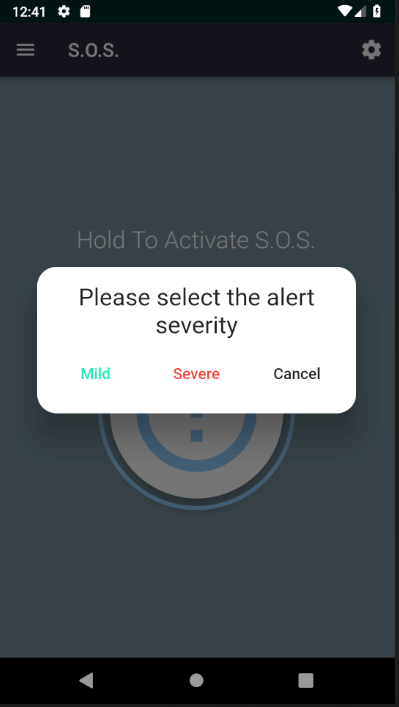
\includegraphics[width=\linewidth]{img/severity.PNG}
  \caption{Client-side prompt requesting that the user select the emergency severity at the end of holding the S.O.S. button.}
\endminipage\hfill
\minipage{0.32\textwidth}
  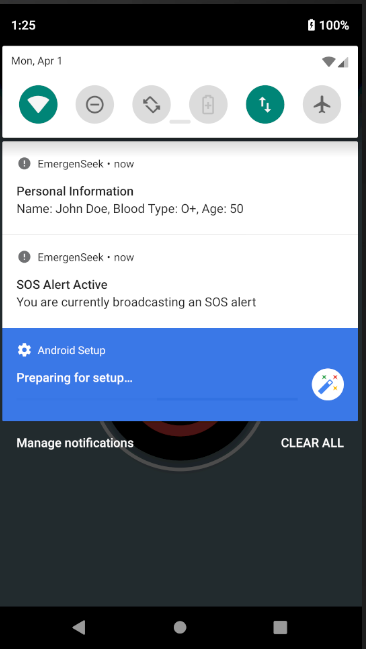
\includegraphics[width=\linewidth]{img/notification.png}
  \caption{Example lockscreen data returned from the API as a result of invoking the S.O.S. button.}
\endminipage\hfill
\minipage{0.32\textwidth}%
  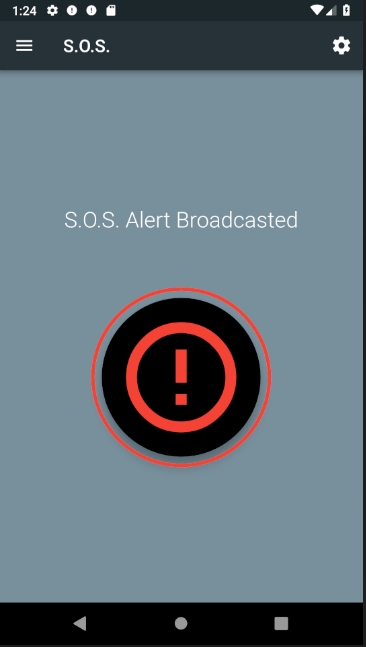
\includegraphics[width=\linewidth]{img/broadcasted.png}
  \caption{The state of the S.O.S. button after being invokved. As long as the button is in an invoked state, lockscreen information will be displayed.}
\endminipage
\end{figure}

\subsection{2 - Emergency service locator}
\par ~ This client feature depends on only one backend Lambda function. On the client side, whenever the user opens the service locator application, a single asynchronous HTTP POST request will be made, containing the user's current location extracted from the device using native permissions. ESServiceLocator will then response with a list of JSON objects each containing information about a hospital or pharmacy. The client will, using the data returned by ESServiceLocator, create a map markers. The markers will then be placed on a Google-style map for the viewing of the user. The Flutter package responsible for friendly displaying of the returned geo-data is a result of the \texttt{google\_maps\_flutter} plugin (\url{https://github.com/flutter/plugins/tree/master/packages/google\_maps\_flutter}).

\begin{figure}[H]
  \centerline{
  	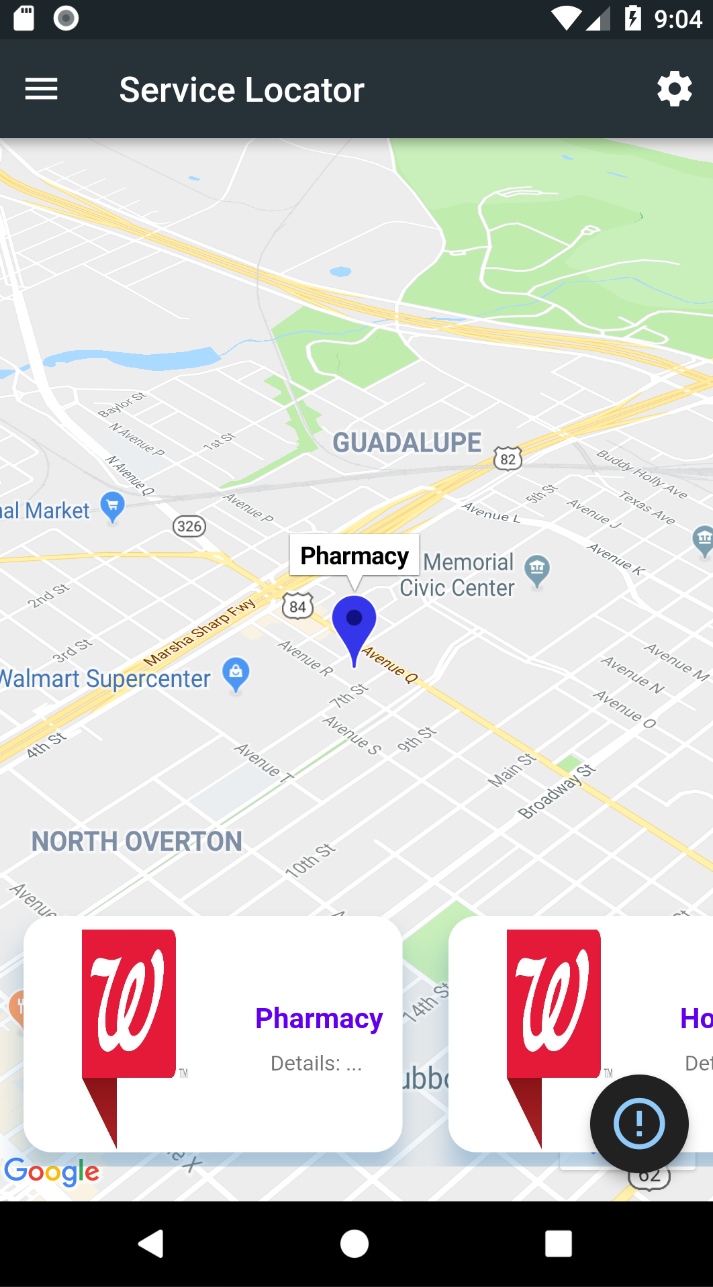
\includegraphics[scale=.8]{img/service-locator.PNG}
  }  
  \caption{Screenshot of the service locator map containing mock data.}
\end{figure}

\subsection{3 - Periodic notifications to contacts (location-based polling)}
\par ~ A note that this feature has not been implemented, but it's implementation details are something that we have discussed since our SRS document. This client feature depends on only one backend lambda function. On the client side, a primitive \texttt{Thread}, provided by the \texttt{threading} package, will start whenever the client first registers for the application and enables the location-based polling feature. By default, the thread will sleep for 24 hours. At the end of the sleep, the client will make a single asynchronous HTTP POST request to ESPollLocation containing the user's id, and their location at the time of the API call.

\subsection{4 - Granular permission definitions for contacts}
\par ~ This client feature depends on one backend Lambda function. On the client side, user's are able to add and removes users from their native contacts book. Each contact is then assigned an alert tier. Depending on their alert tier, depends on how detailed the location information that they receive is. For example, a user assigned alert tier 1 would be able to see  2500 Broadway, Lubbock, TX 79409, USA, but a user assigned a tier 3 alert tier would only see TX, USA.

\begin{figure}[H]
  \centerline{
  	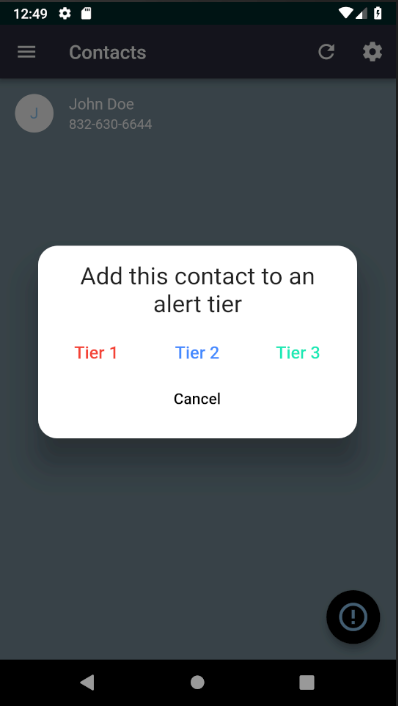
\includegraphics[scale=.8]{img/alert-tier.PNG}
  }  
  \caption{Client-side prompt containing alert tier selection for a single user.}
\end{figure}

\section{Continuous Integration / Continuous Deployment}
\label{sec:cicd}
\par ~ In this section, we will d
% TODO: Add photo of CodeStar pipeline


\begin{thebibliography}{9}
\bibitem{one}
What is the AWS Serverless Application Model (AWS SAM)? --- \url{https://docs.aws.amazon.com/serverless-application-model/latest/developerguide/what-is-sam.html}
\bibitem{two}
TwiML\textsuperscript{TM} for Programmable Voice --- https://www.twilio.com/docs/voice/twiml

\end{thebibliography}
\end{document}

